\documentclass[tikz, border=10pt]{standalone}
\usepackage{amsmath}
\usepackage{amssymb}
\usepackage{bm}
\usetikzlibrary{decorations.pathreplacing, positioning, shapes.geometric, arrows.meta, calc, fit, backgrounds}

\begin{document}

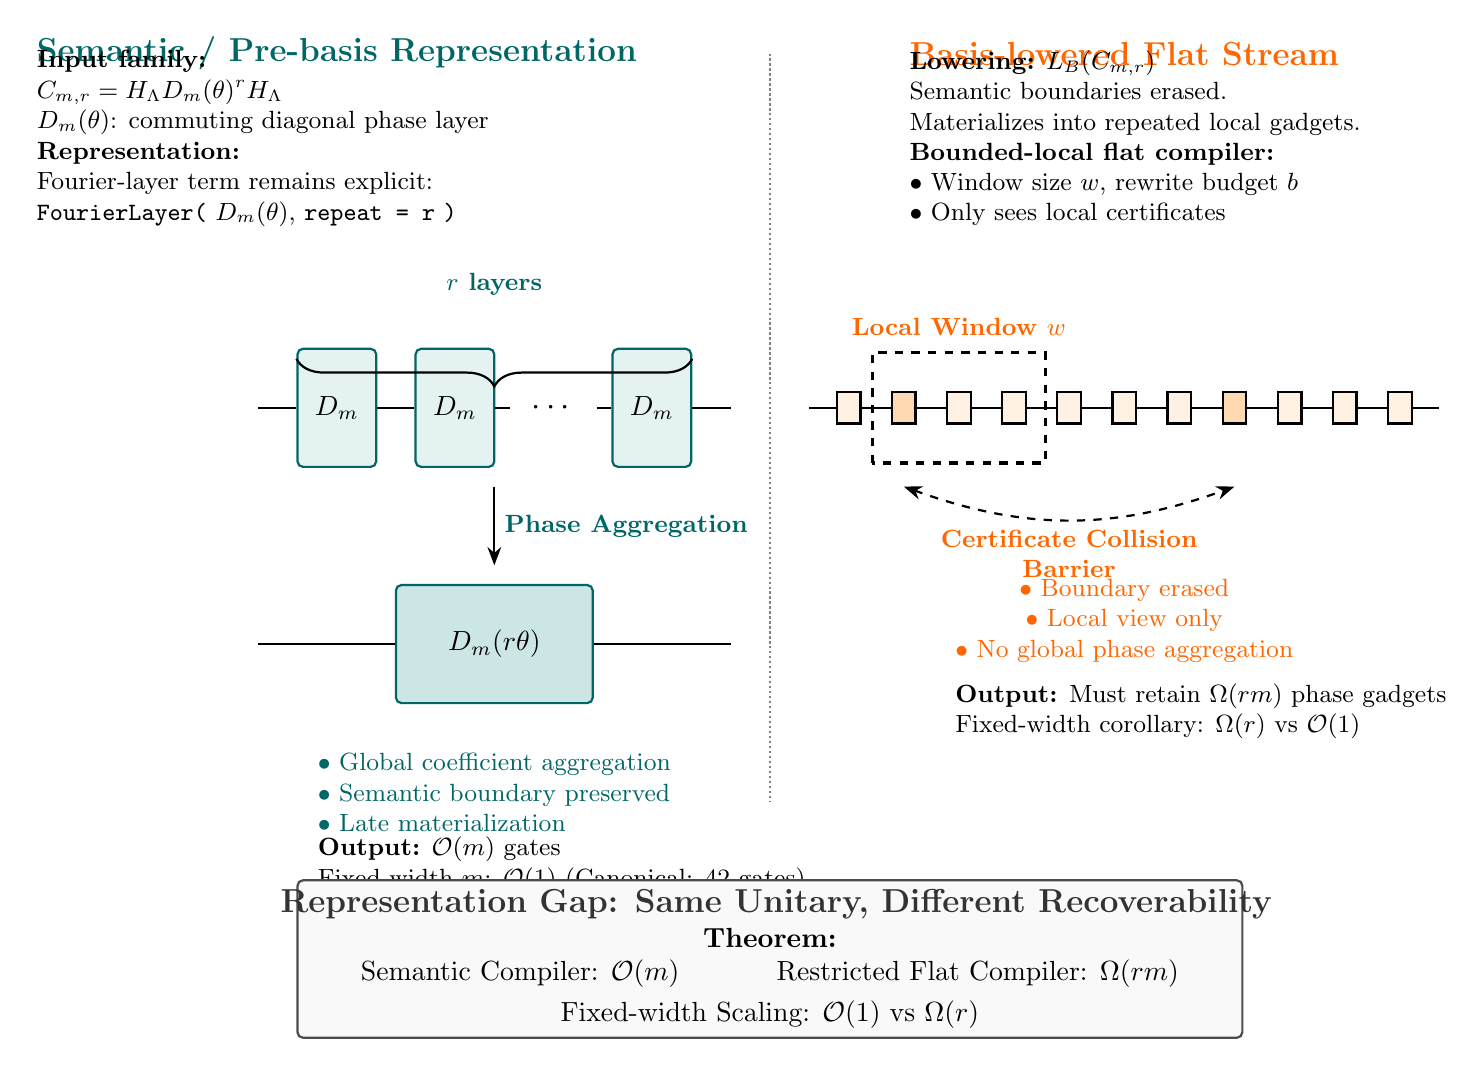
\begin{tikzpicture}[
    font=\sffamily,
    >=Stealth,
    % Color Palette
    semanticColor/.style={draw=teal!80!black, fill=teal!10},
    semanticDark/.style={text=teal!80!black},
    flatColor/.style={draw=orange!80!red, fill=orange!10},
    flatDark/.style={text=orange!80!red},
    % Node Styles
    box/.style={rectangle, rounded corners=2pt, thick, align=center, minimum height=0.8cm},
    gate/.style={rectangle, draw, thick, fill=white, minimum width=0.6cm, minimum height=0.6cm},
    smallgate/.style={rectangle, draw, thick, fill=white, minimum width=0.3cm, minimum height=0.4cm},
    title/.style={font=\large\bfseries},
    subtitle/.style={font=\normalsize\bfseries},
    desc/.style={font=\small, align=left}
]

% =========================================================
% LEFT COLUMN: Semantic / Pre-basis Representation
% =========================================================
\node[title, semanticDark] (leftTitle) at (0, 0) {Semantic / Pre-basis Representation};

% Input
\node[desc, below=0.5cm of leftTitle.west, anchor=west] (leftInput) {
    \textbf{Input family:}\\
    $C_{m,r} = H_\Lambda D_m(\theta)^r H_\Lambda$\\
    $D_m(\theta)$: commuting diagonal phase layer
};

% Representation
\node[desc, below=0.5cm of leftInput.south west, anchor=west] (leftRep) {
    \textbf{Representation:}\\
    Fourier-layer term remains explicit:\\
    \texttt{FourierLayer(} $D_m(\theta)$, \texttt{repeat = r} \texttt{)}
};

% Visual Diagram for Semantic
\coordinate (semStart) at (0, -4.5);
\node[box, semanticColor, minimum width=1cm, minimum height=1.5cm] (d1) at (semStart) {$D_m$};
\node[box, semanticColor, minimum width=1cm, minimum height=1.5cm] (d2) at (1.5, -4.5) {$D_m$};
\node[font=\large] (dots) at (2.75, -4.5) {$\cdots$};
\node[box, semanticColor, minimum width=1cm, minimum height=1.5cm] (dr) at (4, -4.5) {$D_m$};

\draw[thick] (-1, -4.5) -- (d1.west);
\draw[thick] (d1.east) -- (d2.west);
\draw[thick] (d2.east) -- (2.2, -4.5);
\draw[thick] (3.3, -4.5) -- (dr.west);
\draw[thick] (dr.east) -- (5, -4.5);

\draw[decorate,decoration={brace,amplitude=10pt,raise=4pt}, thick, semanticDark] 
    (dr.north east) -- (d1.north west) node[midway, above=15pt, font=\small\bfseries] {$r$ layers};

\draw[->, thick, semanticDark] (2, -5.5) -- (2, -6.5) node[midway, right, font=\small] {\textbf{Phase Aggregation}};

\node[box, semanticColor, minimum width=2.5cm, minimum height=1.5cm, fill=teal!20] (dAgg) at (2, -7.5) {$D_m(r\theta)$};
\draw[thick] (-1, -7.5) -- (dAgg.west);
\draw[thick] (dAgg.east) -- (5, -7.5);

% Left Keywords
\node[desc, semanticDark, below=0.5cm of dAgg] (leftKeywords) {
    $\bullet$ Global coefficient aggregation\\
    $\bullet$ Semantic boundary preserved\\
    $\bullet$ Late materialization
};

% Left Output
\node[desc, below=0.3cm of leftKeywords.south west, anchor=west] (leftOutput) {
    \textbf{Output:} $\mathcal{O}(m)$ gates\\
    Fixed-width $m$: $\mathcal{O}(1)$ (Canonical: 42 gates)
};


% =========================================================
% RIGHT COLUMN: Basis-lowered Flat Stream
% =========================================================
\node[title, flatDark] (rightTitle) at (10, 0) {Basis-lowered Flat Stream};

% Input
\node[desc, below=0.5cm of rightTitle.west, anchor=west] (rightInput) {
    \textbf{Lowering:} $L_B(C_{m,r})$\\
    Semantic boundaries erased.\\
    Materializes into repeated local gadgets.
};

% Compiler constraints
\node[desc, below=0.5cm of rightInput.south west, anchor=west] (rightComp) {
    \textbf{Bounded-local flat compiler:}\\
    $\bullet$ Window size $w$, rewrite budget $b$\\
    $\bullet$ Only sees local certificates
};

% Visual Diagram for Flat Stream
\coordinate (flatStart) at (6, -4.5);
\draw[thick] (flatStart) -- (14, -4.5);

% Draw many small gates
\foreach \x in {6.5, 7.2, 7.9, 8.6, 9.3, 10.0, 10.7, 11.4, 12.1, 12.8, 13.5} {
    \node[smallgate, fill=orange!10] at (\x, -4.5) {};
}
\node[smallgate, fill=orange!30] at (7.2, -4.5) {};
\node[smallgate, fill=orange!30] at (11.4, -4.5) {};

% Local Window
\draw[dashed, very thick, flatDark] (6.8, -5.2) rectangle (9.0, -3.8);
\node[flatDark, font=\small\bfseries, above=0.1cm of {(7.9, -3.8)}] {Local Window $w$};

% Certificate collision pointing
\draw[<->, dashed, thick, flatDark] (7.2, -5.5) to[bend right=20] node[midway, below, align=center, font=\small\bfseries] {Certificate Collision\\Barrier} (11.4, -5.5);

% Right Keywords
\node[desc, flatDark, align=center] (rightKeywords) at (10, -7.2) {
    $\bullet$ Boundary erased\\
    $\bullet$ Local view only\\
    $\bullet$ No global phase aggregation
};

% Right Output
\node[desc, below=0.5cm of rightKeywords.south west, anchor=west] (rightOutput) {
    \textbf{Output:} Must retain $\Omega(rm)$ phase gadgets\\
    Fixed-width corollary: $\Omega(r)$ vs $\mathcal{O}(1)$
};

% =========================================================
% DIVIDER LINE
% =========================================================
\draw[densely dotted, thick, gray] (5.5, 0) -- (5.5, -9.5);

% =========================================================
% BOTTOM CONCLUSION BOX
% =========================================================
\node[box, draw=black!70, fill=gray!5, minimum width=12cm, minimum height=2cm] (conclusion) at (5.5, -11.5) {};

\node[font=\large\bfseries, text=black!80, anchor=north] at (conclusion.north) {\vspace{0.2cm} Representation Gap: Same Unitary, Different Recoverability};

\node[align=center, font=\normalsize, below=0.5cm of conclusion.north] {
    \textbf{Theorem:}\\
    Semantic Compiler: $\mathcal{O}(m)$ \hspace{1cm} Restricted Flat Compiler: $\Omega(rm)$\\[0.1cm]
    Fixed-width Scaling: $\mathcal{O}(1)$ vs $\Omega(r)$
};

\end{tikzpicture}

\end{document}